\documentclass[a4paper]{article}
\usepackage{tikz}
\usepackage{geometry}
\usepackage{graphicx}
\usepackage{natbib}
\usepackage{amsmath}
\usepackage{amssymb}
\usepackage{amsthm}
\usepackage{paralist}
\usepackage{epstopdf}
\usepackage{tabularx}
\usepackage{longtable}
\usepackage{multirow}
\usepackage{multicol}
\usepackage[hidelinks]{hyperref}
\usepackage{fancyvrb}
\usepackage{algorithm}
\usepackage{algorithmic}
\usepackage{float}
\usepackage{paralist}
%\usepackage[svgname]{xcolor}
\usepackage{enumerate}
\usepackage{array}
\usepackage{times}
\usepackage{url}
\usepackage{fancyhdr}
\usepackage{comment}
\usepackage{environ}
\usepackage{times}
\usepackage{textcomp}
\usepackage{caption}
\usepackage{bbm}


\urlstyle{rm}

\setlength\parindent{0pt} % Removes all indentation from paragraphs
\theoremstyle{definition}
\newtheorem{definition}{Definition}[]
\newtheorem{conjecture}{Conjecture}[]
\newtheorem{example}{Example}[]
\newtheorem{theorem}{Theorem}[]
\newtheorem{lemma}{Lemma}
\newtheorem{proposition}{Proposition}
\newtheorem{corollary}{Corollary}

\floatname{algorithm}{Procedure}
\renewcommand{\algorithmicrequire}{\textbf{Input:}}
\renewcommand{\algorithmicensure}{\textbf{Output:}}
\newcommand{\abs}[1]{\lvert#1\rvert}
\newcommand{\norm}[1]{\lVert#1\rVert}
\newcommand{\RR}{\mathbb{R}}
\newcommand{\CC}{\mathbb{C}}
\newcommand{\Nat}{\mathbb{N}}
\newcommand{\br}[1]{\{#1\}}
\DeclareMathOperator*{\argmin}{arg\,min}
\DeclareMathOperator*{\argmax}{arg\,max}
\renewcommand{\qedsymbol}{$\blacksquare$}

\definecolor{dkgreen}{rgb}{0,0.6,0}
\definecolor{gray}{rgb}{0.5,0.5,0.5}
\definecolor{mauve}{rgb}{0.58,0,0.82}

\definecolor{C0}{HTML}{1F77B4}
\definecolor{C1}{HTML}{FF7F0E}
\definecolor{C2}{HTML}{2ca02c}
\definecolor{C3}{HTML}{d62728}
\definecolor{C4}{HTML}{9467bd}
\definecolor{C5}{HTML}{8c564b}
\definecolor{C6}{HTML}{e377c2}
\definecolor{C7}{HTML}{7F7F7F}
\definecolor{C8}{HTML}{bcbd22}
\definecolor{C9}{HTML}{17BECF}

\newcommand{\Var}{\mathrm{Var}}
\newcommand{\Cov}{\mathrm{Cov}}
\newcommand{\sgn}{\mathrm{sgn}}

\newcommand{\vc}[1]{\boldsymbol{#1}}
\newcommand{\xv}{\vc{x}}
\newcommand{\Sigmav}{\vc{\Sigma}}
\newcommand{\alphav}{\vc{\alpha}}
\newcommand{\muv}{\vc{\mu}}

\newcommand{\red}[1]{\textcolor{red}{#1}}

\def\x{\mathbf x}
\def\y{\mathbf y}
\def\w{\mathbf w}
\def\v{\mathbf v}
\def\E{\mathbb E}
\def\R{\mathbb R}
\def\V{\mathbb V}
\def\ind{\mathbbm 1}

% TO SHOW SOLUTIONS, include following (else comment out):
\newenvironment{soln}{
    \leavevmode\color{blue}\ignorespaces
}{}


\hypersetup{
%    colorlinks,
    linkcolor={red!50!black},
    citecolor={blue!50!black},
    urlcolor={blue!80!black}
}

\geometry{
  top=1in,            % <-- you want to adjust this
  inner=1in,
  outer=1in,
  bottom=1in,
  headheight=3em,       % <-- and this
  headsep=2em,          % <-- and this
  footskip=3em,
}


\pagestyle{fancyplain}
\lhead{\fancyplain{}{Homework 6}}
\rhead{\fancyplain{}{CS 760 Machine Learning}}
\cfoot{\thepage}

\title{\textsc{Homework 6}} % Title

%%% NOTE:  Replace 'NAME HERE' etc., and delete any "\red{}" wrappers (so it won't show up as red)

\author{
Arnav Sharma\\
9074042756\\
} 

\date{}

\begin{document}

\maketitle 


\textbf{Instructions:} 
You can choose any programming language as long as you implement the algorithm from scratch. Use this latex file as a template to develop your homework.
Submit your homework on time as a single pdf file to Canvas.
Please check Piazza for updates about the homework.\\


\section{Kernel SVM [30pts]}
Consider the following kernel function defined over $\mathbf z,\mathbf z'\in Z$, where $Z$ is some set:
\[
\kappa(\mathbf z,\mathbf z')=\begin{cases}
    1 \quad \mathrm{if }\;\; \mathbf z=\mathbf z',\\
0\quad \mathrm{otherwise}.
\end{cases}
\]
\begin{enumerate}
    \item (10 pts) Prove that for any positive integer $m$, any $\mathbf z_1, \ldots,\mathbf z_m \in Z$, the $m\times m$ kernel matrix $\mathbf K = [\mathbf K_{ij} ]$ is
positive semi-definite, where $\mathbf K_{ij} = \kappa(\mathbf z_i
, \mathbf z_j )$ for $i, j = 1 \ldots m$. (Let us assume that for $i \neq j$, we have
$\mathbf z_i \neq \mathbf z_j$) Hint: An  $m\times m$  matrix $K $ is positive semi-definite if  $\forall \mathbf u\in \R^d: \mathbf u^\top \mathbf K\mathbf u\geq 0$.
\begin{soln}
    \\We're Given: 
    \[ \mathbf K = [ \mathbf K_{ij} ] \quad \& \quad  \mathbf z_i \neq \mathbf z_j \;\;\mathrm{ if }\;\; \mathbf i \neq \mathbf j \]
    \[ \implies \mathbf K = [ \kappa(\mathbf z_i,\mathbf z_j)  ] \quad \& \quad  \mathbf z_i \neq \mathbf z_j \;\;\mathrm{ if }\;\; \mathbf i \neq \mathbf j \]
    \[ \implies \mathbf K_{ij}=\begin{cases}
                1 \quad \mathrm{if }\;\; \mathbf i=\mathbf j,\\
                0\quad \mathrm{otherwise}.\end{cases} 
    \]
    \\ Since $\mathbf K$ is an $m \times m$ Matrix,
    \[ \implies \mathbf K = \mathbf{I_{m \times m}} \]
    \\ To Prove:
    \[ \mathbf x^\top \mathbf K\mathbf x\geq 0 \:\: \forall \mathbf x\in \R^m \]
    \[ \implies x^\top \mathbf K\mathbf x = \mathbf x^\top \mathbf \mathbf{I_{m \times m}}\mathbf x \]
    \[ \implies x^\top \mathbf K\mathbf x = \begin{bmatrix} \sum_{l=1}^{m} \mathbf x_l I_{l, 1} \:\: \sum_{l=1}^{m} \mathbf x_l I_{l, 2} \:\: \dots \:\: \sum_{l=1}^{m} \mathbf x_l I_{l, m} \end{bmatrix} \mathbf x \]
    \\ Since $I_{i, j} = 1$ if i=j, else $I_{i, j} = 0$
    \[ \forall i \in [m], \sum_{l=1}^{m}\mathbf{x}_l I_{l, i} =  0 + 0 + \dots + \mathbf{x_i} + \dots + 0 = \mathbf{x_i} \]
    \[ \implies x^\top \mathbf K\mathbf x = \begin{bmatrix} x_1 \:\: x_2 \:\: \dots \:\: x_m \end{bmatrix} \mathbf x \]
    \[ \implies x^\top \mathbf K\mathbf x = \mathbf x^\top \mathbf x \]
    \\Since $\mathbf x^\top \mathbf x = \left \| x \right \|^{2} $ which is $ \geq 0 \forall x \in R^m $
    \[ \implies x^\top \mathbf K\mathbf x \geq 0\:\: \forall \mathbf x\in \R^m \]
    \\ Therefore, proved that $K$ is a positive semi-definite matrix

\end{soln}
\item (10 pts) Given a training set $(\mathbf z_1, y_1), \ldots,(\mathbf z_n, y_n)$ with binary labels, the dual SVM problem with the above
kernel $\kappa$ will have parameters $a_1, \ldots, a_n,b \in \R$. (Let us assume that for $i \neq j$, we have
$\mathbf z_i \neq \mathbf z_j$) The predictor
for input $\mathbf z$ takes the form
\[
f(\mathbf z)=\sum_{i=1}^na_iy_i\kappa(\mathbf z_i,z) +b\;.
\]
Recall that the label prediction is $\mathrm{sgn}(f(\mathbf z))$. Prove that there exist $a_1, \ldots, a_n, b$ such that $f$ correctly separates
the training set. In other words, $\kappa$ induces a feature space rich enough such that in it, any training set can be linearly separated.
\begin{soln}
    \\Let $\mathbf{z_k}$ be an arbitrary point in our training set such that $k \in [1,\: n]$. In order for our predictor to correctly predict the label of this arbitrary point, it must match the sign of the chosen training point, i.e.
    \[ \mathrm{sgn}(f(\mathbf {z_k})) = \mathrm{sgn}(y_k)\]
    \\ where, 
    \[ f(\mathbf z)=\sum_{i=1}^na_iy_i\kappa(\mathbf z_i,z) +b\; \]
    \[ f(\mathbf {z_k})=\sum_{i=1}^na_iy_i\kappa(\mathbf z_i,z_k) +b\; \]\
    \[ f(\mathbf {z_k})=\sum_{i \neq k}a_iy_i\kappa(\mathbf z_i,z_k) + a_ky_k\kappa(\mathbf z_k,z_k) +b\; \]
    \\According to the definition of our kernel,
    \[ f(\mathbf {z_k})=\sum_{i \neq k}a_iy_i(0 )+ a_ky_k(1) +b\; \]
    \[ f(\mathbf {z_k})= a_ky_k +b\; \]
    \\ Since $\mathrm{sgn}(f(\mathbf {z_k}))$ should be the same as $\mathrm{sgn}(y_k)$, we want:
    \[ \mathrm{sgn}(a_ky_k +b) = \mathrm{sgn}(y_k)\; \]
    \\ Therefore, any $a_1, \ldots, a_n, b$, that follow the condition above will be able to correctly separate the training set and therefore correctly predict all the examples.
    \\ Taking the example of b = 0, $a_1, \ldots, a_n = 1$, we have 
    \[ \mathrm{sgn}(1 \: (y_k) +0) = \mathrm{sgn}(y_k)\; \forall k \in [1, n]\]
    \\Since the equation above is an identity, we can show that for $a_1, \ldots, a_n = 1$, $b = 0$, our kernel will be able to separate out all the training examples successfully for atleast one set of
    $a_1, \ldots, a_n, b$
\end{soln}
\item (10 pts) How does that $f$ predict input $\mathbf z$ that is not in the training set?
\begin{soln}
    \\Since our predictor takes the form:
    \[ f(\mathbf z)=\sum_{i=1}^na_iy_i\kappa(\mathbf z_i,z) +b\; \]
    We need to consider two cases ( when $z = z_i \;\;\exists\: i \in [n]$ and when $z \neq z_i \;\;\forall\: i \in [n]\;\;$)
    \\If $\mathbf z$ is not in our training set, that means that $z \neq z_i \;\;\forall\: i \in [n]$, i.e. by the definition of our Kernel,
    \[ f(\mathbf z)=\sum_{i=1}^na_iy_i\kappa(\mathbf z_i,z) +b\; = \sum_{i=1}^na_iy_i(0) +b\]
    \[ = b\]
    \\ $\therefore\:,$ we will predict such a test example using the following criteria:
    \[ \mathrm{sgn}(f(\mathbf z)) = \mathrm{sgn}(b)\]
    \\ This will result in the kernel guessing the value of $\mathrm{sgn}(f(\mathbf z))$, based on the sign of $b$, i.e. all examples not in the training set will be classified with the same label.
\end{soln}
\end{enumerate}

Comment: One useful property of kernel functions is that the input space $Z$ does not need to be a vector space; in
other words, $\mathbf z$ does not need to be a feature vector. For all we know, $Z$ can be all the turkeys in the world. As long as we
can compute $\kappa(\mathbf z, \mathbf z')$, kernel SVM works on turkeys.

\section{Chow-Liu Algorithm [30 pts]}
Suppose we wish to construct a directed graphical model for 3 features $X$, $Y$, and $Z$ using the Chow-Liu algorithm. We are given data from 100 independent experiments where each feature is binary and takes value $T$ or $F$. Below is a table summarizing the observations of the experiment:

\begin{table}[H]
        \centering
                \begin{tabular}{cccc}
                           $X$ & $Y$ & $Z$ & Count \\
                                \hline
                                T & T & T & 36 \\
                                \hline
                                T & T & F & 4 \\
                                \hline
                                T & F & T & 2 \\
                                \hline
                                T & F & F & 8 \\
                                \hline
                                F & T & T & 9 \\
                                \hline
                                F & T & F & 1 \\
                                \hline
                                F & F & T & 8 \\
                                \hline
                                F & F & F & 32 \\
                                \hline
                \end{tabular}
\end{table}

\begin{enumerate}
	\item Compute the mutual information $I(X, Y)$ based on the frequencies observed in the data. (5 pts)
	\begin{soln}
        \[  I(X, Y) = \sum_{x \in X} \sum_{y \in Y} P_{X,Y}[x, y]\:log(\cfrac{P_{X,Y}[x, y]}{P_X[x]P_Y[y]})  \]
        \[  I(X, Y) = \]
        \[ P_{X,Y}[x=F, y=F]\:log(\cfrac{P_{X,Y}[x=F, y=F]}{P_X[x=F]P_Y[y=F]}) + P_{X,Y}[x=F, y=T]\:log(\cfrac{P_{X,Y}[x=F, y=T]}{P_X[x=F]P_Y[y=T]})\]
        \[  + P_{X,Y}[x=T, y=F]\:log(\cfrac{P_{X,Y}[x=T, y=F]}{P_X[x=T]P_Y[y=F]}) + P_{X,Y}[x=T, y=T]\:log(\cfrac{P_{X,Y}[x=T, y=T]}{P_X[x=T]P_Y[y=T]})\]
        \[  = \frac{40}{100}\:log(\cfrac{\frac{40}{100}}{\frac{50}{100}\frac{50}{100}}) + \frac{10}{100}\:log(\cfrac{\frac{10}{100}}{\frac{50}{100}\frac{50}{100}})\]
        \[  + \frac{10}{100}\:log(\cfrac{\frac{10}{100}}{\frac{50}{100}\frac{50}{100}}) + \frac{40}{100}\:log(\cfrac{\frac{40}{100}}{\frac{50}{100}\frac{50}{100}})\]
        \[  = \frac{80}{100}\:log(\cfrac{\frac{40}{100}}{\frac{50}{100}\frac{50}{100}}) + \frac{20}{100}\:log(\cfrac{\frac{10}{100}}{\frac{50}{100}\frac{50}{100}})\]
        \[  = \cfrac{1}{5} (4log(\cfrac{\frac{40}{100}}{\frac{50}{100}\frac{50}{100}}) + log(\cfrac{\frac{10}{100}}{\frac{50}{100}\frac{50}{100}})) \]
        \[  = \cfrac{1}{5} (4\times0.6781 - 1.322) = \cfrac{1}{5} (2.7124 - 1.322)\]
        \[  = \cfrac{1.3904}{5} \]
        \[  = 0.27808\]
    \end{soln}
	\item Compute the mutual information $I(X, Z)$ based on the frequencies observed in the data. (5 pts)
	\begin{soln}
        \[  I(X, Z) = \sum_{x \in X} \sum_{z \in Z} P_{X,Z}[x, z]\:log(\cfrac{P_{X,Z}[x, z]}{P_X[x]P_Z[z]})  \]
        \[  I(X, Z) = \]
        \[ P_{X,Z}[x=F, z=F]\:log(\cfrac{P_{X,Z}[x=F, z=F]}{P_X[x=F]P_Z[z=F]}) + P_{X,Z}[x=F, z=T]\:log(\cfrac{P_{X,Z}[x=F, y=T]}{P_X[x=F]P_Z[z=T]})\]
        \[  + P_{X,Z}[x=T, z=F]\:log(\cfrac{P_{X,Z}[x=T, z=F]}{P_X[x=T]P_Z[z=F]}) + P_{X,Z}[x=T, z=T]\:log(\cfrac{P_{X,Z}[x=T, z=T]}{P_X[x=T]P_Z[z=T]})\]
        \[  = \frac{33}{100}\:log(\cfrac{\frac{33}{100}}{\frac{50}{100}\frac{45}{100}}) + \frac{17}{100}\:log(\cfrac{\frac{17}{100}}{\frac{50}{100}\frac{55}{100}})\]
        \[  + \frac{12}{100}\:log(\cfrac{\frac{12}{100}}{\frac{50}{100}\frac{45}{100}}) + \frac{38}{100}\:log(\cfrac{\frac{38}{100}}{\frac{50}{100}\frac{55}{100}})\]
        \[  = 0.33log(\cfrac{22}{15}) + 0.17log(\cfrac{34}{55}) + 0.12log(\cfrac{8}{15}) + 0.38log(\cfrac{76}{55}) \]
        \[  = 0.182325 - 0.117963 - 0.108828 + 0.177308\]
        \[  = 0.132842 \]
    \end{soln}
	\item Compute the mutual information $I(Z, Y)$ based on the frequencies observed in the data. (5 pts)
	\begin{soln}
        \[  I(Z, Y) = \sum_{z \in Z} \sum_{y \in Y} P_{Z,Y}[z, y]\:log(\cfrac{P_{Z,Y}[z, y]}{P_Z[z]P_Y[y]})  \]
        \[  I(Z, Y) = \]
        \[ P_{Z,Y}[z=F, y=F]\:log(\cfrac{P_{Z,Y}[z=F, y=F]}{P_Z[z=F]P_Y[y=F]}) + P_{Z,Y}[z=F, y=T]\:log(\cfrac{P_{Z,Y}[z=F, y=T]}{P_Z[z=F]P_Y[y=T]})\]
        \[  + P_{Z,Y}[z=T, y=F]\:log(\cfrac{P_{Z,Y}[z=T, y=F]}{P_Z[z=T]P_Y[y=F]}) + P_{Z,Y}[z=T, y=T]\:log(\cfrac{P_{Z,Y}[z=T, y=T]}{P_Z[z=T]P_Y[y=T]})\]
        \[  = \frac{40}{100}\:log(\cfrac{\frac{40}{100}}{\frac{45}{100}\frac{50}{100}}) + \frac{5}{100}\:log(\cfrac{\frac{5}{100}}{\frac{45}{100}\frac{50}{100}})\]
        \[  + \frac{10}{100}\:log(\cfrac{\frac{10}{100}}{\frac{55}{100}\frac{50}{100}}) + \frac{45}{100}\:log(\cfrac{\frac{45}{100}}{\frac{55}{100}\frac{50}{100}})\]
        \[  = 0.4log(\cfrac{16}{9}) + 0.05log(\cfrac{2}{9}) + 0.1log(\cfrac{4}{11}) + 0.45log(\cfrac{18}{11}) \]
        \[  = 0.332 - 0.1085 - 0.14594 +  0.319725\]
        \[  = 0.397285 \]
    \end{soln}
	\item Which undirected edges will be selected by the Chow-Liu algorithm as the maximum spanning tree? (5 pts)
	\begin{soln}
        The undirected edges between $(Z, Y)$ and the between $(X, Y)$ will be the ones slecedted as the maximum spanning tree.
    \end{soln}
	\item Root your tree at node $X$, and assign directions to the selected edges. (10 pts)
	\begin{soln}
        \\Starting at node X, an edge can go from vertex $X$ into vertex $Y$, and a second edge from vertex $Y$ intwo vertex $Z$.
    \end{soln}
\end{enumerate}

\section{Game of Classifiers [60pts]}
\subsection{Implementation}
Implement the following models in the choice of your programming language. Include slack variables in SVM implementation if needed. You can use autograd features of PyTorch, TensorFlow, etc., or derive gradients on your own (but do not use inbuilt models for SVM, Kernel SVM, and Logistic Regression from libraries).
\begin{itemize}
    \item Implement Linear SVM (without kernels).
    \item Implement Kernel SVM, with options for linear, rbf, and polynomial kernels. You should keep the kernel parameters tunable (e.g., do not fix the degree of polynomial kernels but keep it as a variable and play with different values of it.) Is Linear SVM a special case of Kernel SVMs?
\item Implement Logistic Regression with and without kernels (use same kernels as above).
\end{itemize}
\subsection{ Synthetic Dataset-1 (20 pts)}
Generate a 2-D dataset as follows:
Let $\mu = 2.5$ and $\mathbf I_2$ be the $2 \times 2$ identity matrix. Generate points for the positive and negative classes, respectively
from $\mathcal{N} ([\mu, 0], \mathbf I_2)$, and $\mathcal{N} ([-\mu, 0], \mathbf I_2)$. For each class, generate 750 points (1500 in total). Randomly create train, validation, and test splits of 1000, 250, and 250 points, respectively. Do the following with this dataset:
\begin{enumerate}
    \item  (5 pts) Train your Linear SVM, Logistic Regression models and report decision boundaries and test accuracies.
    \begin{soln}
        \\ {\fontsize{10pt}{12pt}\selectfont Linear Logistic Regression:} 
        \\ Test accuracy = 98.8\%
        \\ Decision Boundary:
        \begin{figure}[H]
            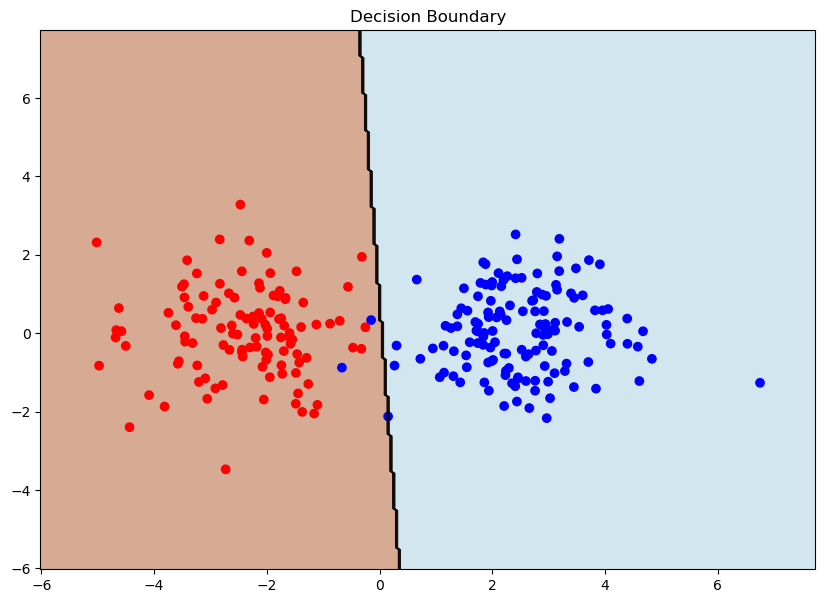
\includegraphics[width=\textwidth]{images/gaussian-linear-lr.png}
            \caption{ Linear Regression decision boundary on test set}
        \end{figure}
        {\fontsize{10pt}{12pt}\selectfont Linear SVM:} 
        \\ Test accuracy = 98.8\%
        \\ Decision Boundary:
        \begin{figure}[H]
            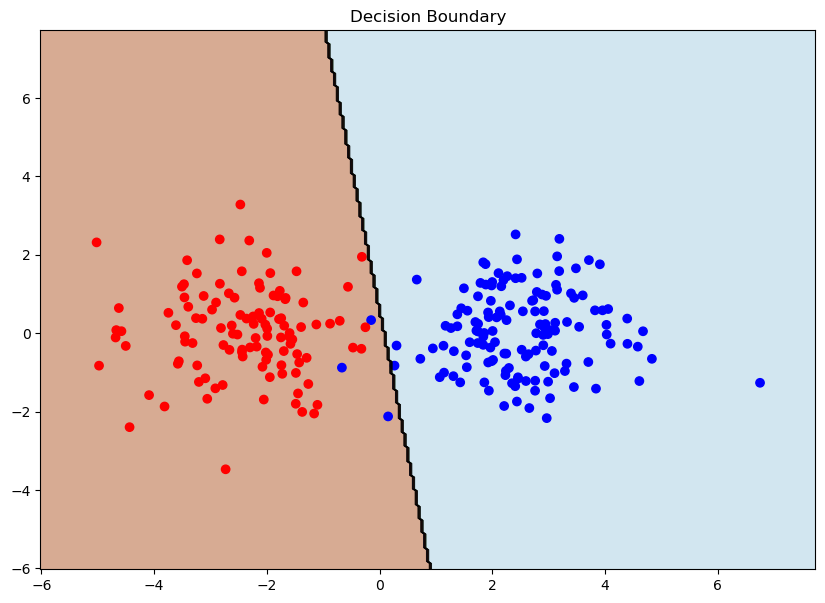
\includegraphics[width=\textwidth]{images/gaussian-linear-svm.png}
            \caption{ Linear Regression decision boundary on test set}
        \end{figure}
    \end{soln}
\item (5 pts) Show the decision boundaries with $k$-NN and Naive Bayes Classifiers. (You can use library implementations or implement from scratch. Figure out the hyper-parameters using the validation set.)
\begin{soln}
    \\ {\fontsize{10pt}{12pt}\selectfont $k$-NN:}
    \\ I chose k = 3 for my $k$-NN model. As increasing k beyond 3 resulted in diminishing returns on accuracy increase.  
    \\ Test accuracy = 99.2\%
    \\ Decision Boundary:
    \begin{figure}[H]
        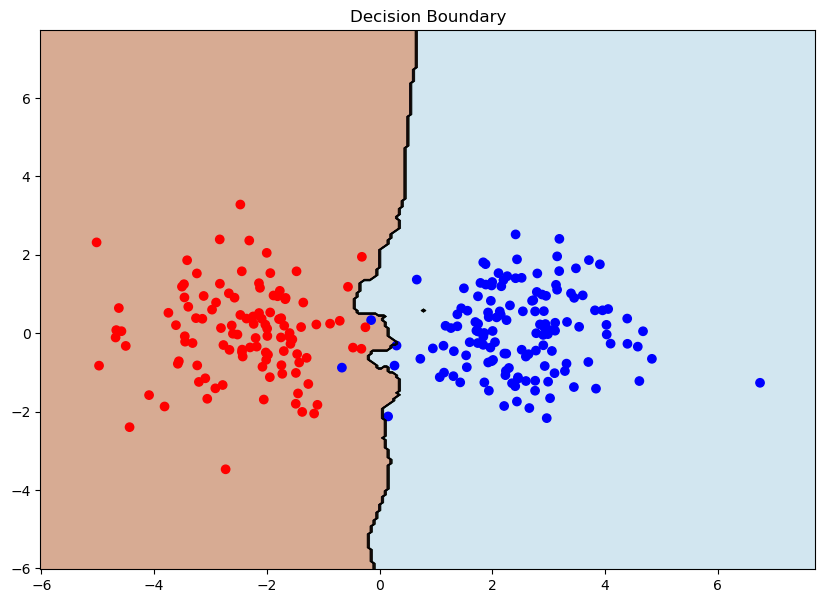
\includegraphics[width=\textwidth]{images/gaussian-knn.png}
        \caption{ $k$-NN decision boundary on test set}
    \end{figure}
    {\fontsize{10pt}{12pt}\selectfont Gausian Naive Bayes Model:} 
    \\ Test accuracy = 99.2\%
    \\ Decision Boundary:
    \begin{figure}[H]
        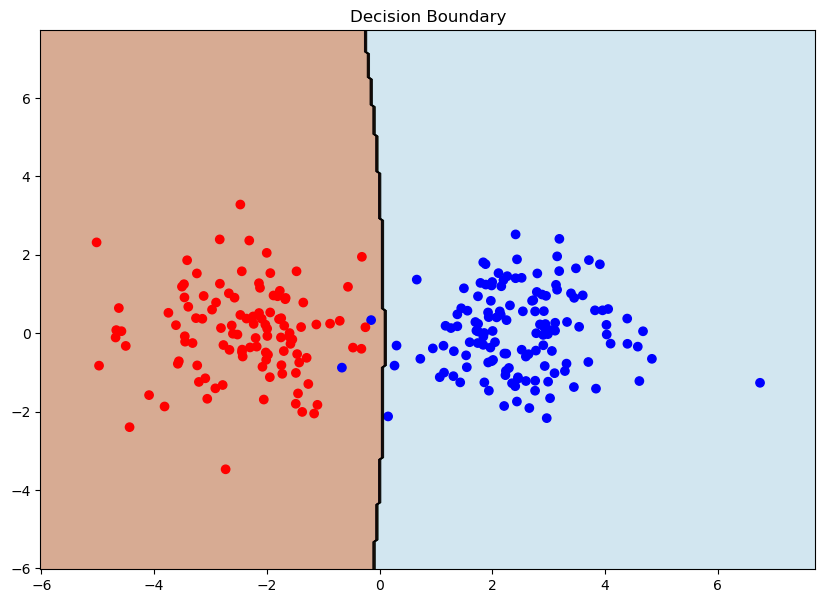
\includegraphics[width=\textwidth]{images/gaussian-naive-bayes.png}
        \caption{ Gausian Naive Bayes decision boundary on test set}
    \end{figure}
\end{soln}
\item (5 pts) Repeat the process by varying $\mu$ from 1.0 to 2.4 with a step size of 0.2 for each value of $\mu$ to obtain test
accuracies of the models and plot ( $\mu$ on $x$-axis and test accuracy on $y$-axis). (You will have a curve for
each of the 4-classifiers mentioned above.)
\begin{soln}
    \begin{figure}[H]
        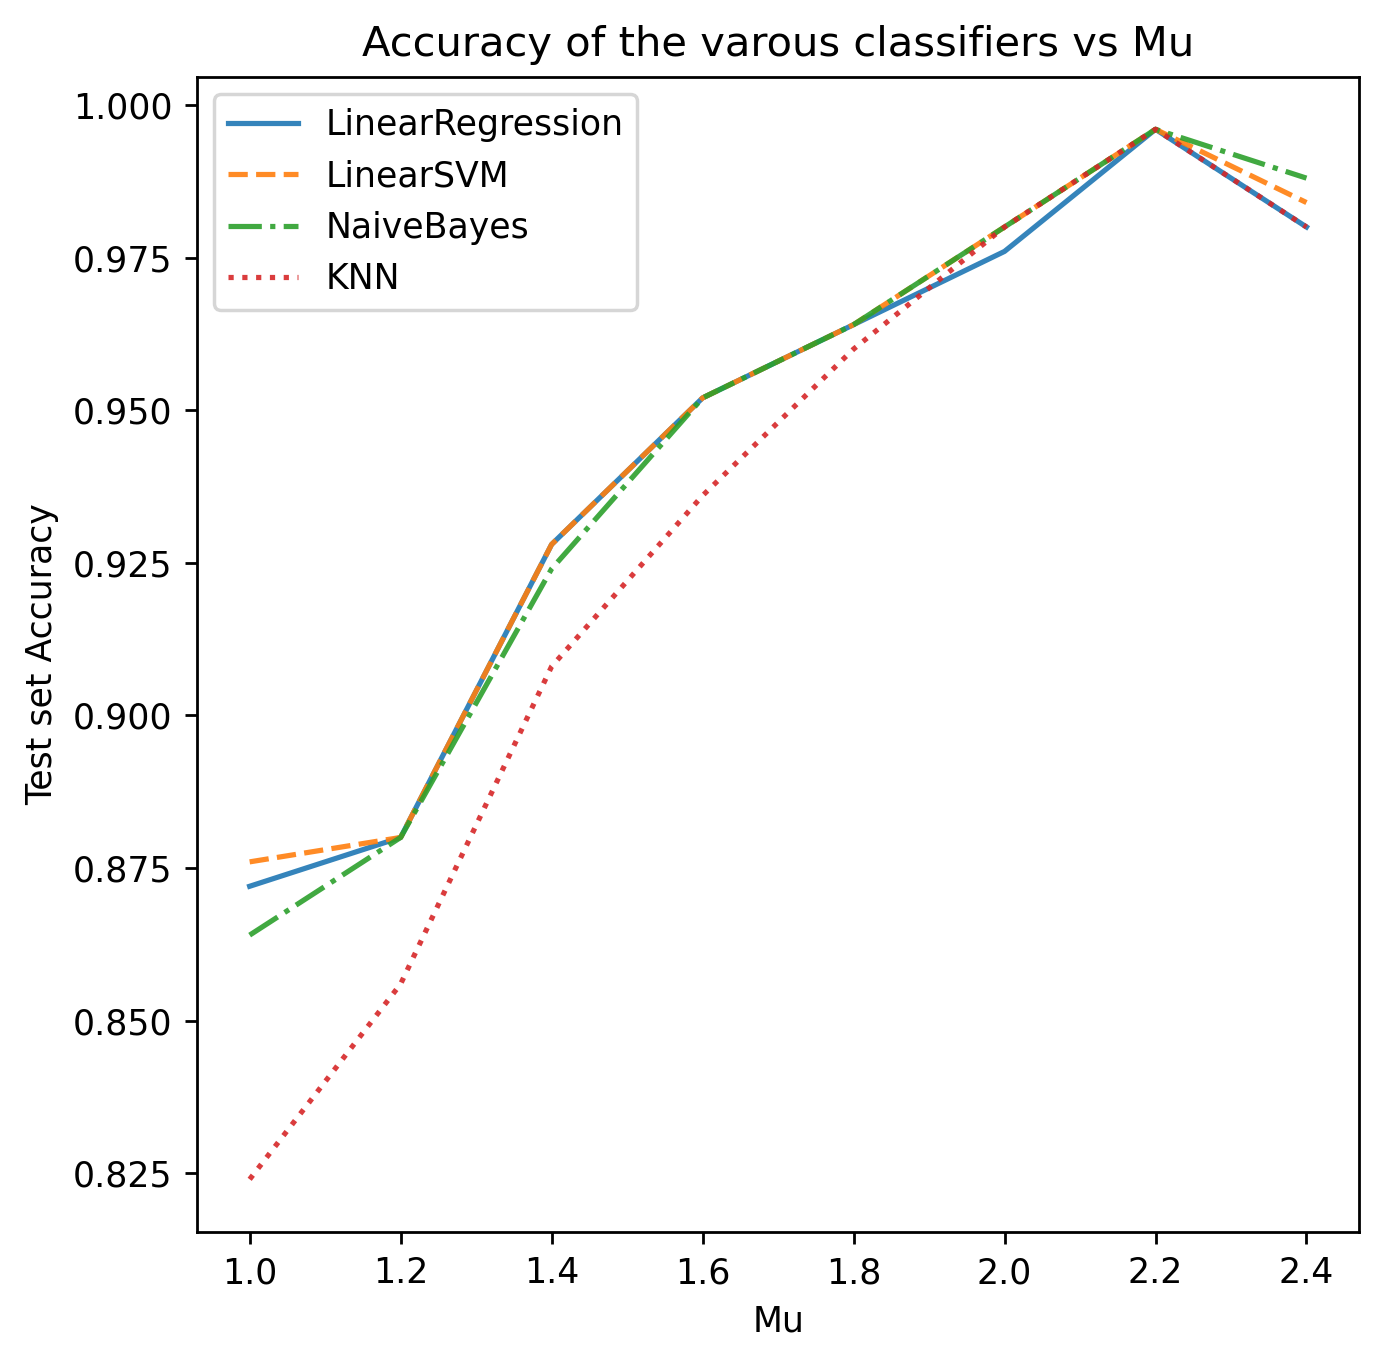
\includegraphics[width=\textwidth]{images/test_acc_vs_mu.png}
        \caption{ Test set accuracy for the various models mentioned above as mu increases from 1.0 to 2.4}
    \end{figure}
\end{soln}
\item (5 pts) What are your conclusions from this exercise?
\end{enumerate}
\subsection{Synthetic Dataset-2 (20 pts)}
Generate 1500 data points from the 2-D circles dataset of sklearn:\begin{verbatim}
    sklearn.datasets.make_circles
\end{verbatim}
Randomly create train, validation, and test splits of 1000, 250, and 250 points, respectively. Evaluate the above classifiers in this setting.
\begin{enumerate}
    \item ( 5 pts) Show decision boundaries for Linear SVM and Logistic Regression classifiers.
    \begin{soln}
        \\ {\fontsize{10pt}{12pt}\selectfont Linear Logistic Regression:} 
        \\ Test accuracy = 48.8 \%
        \\ Decision Boundary:
        \begin{figure}[H]
            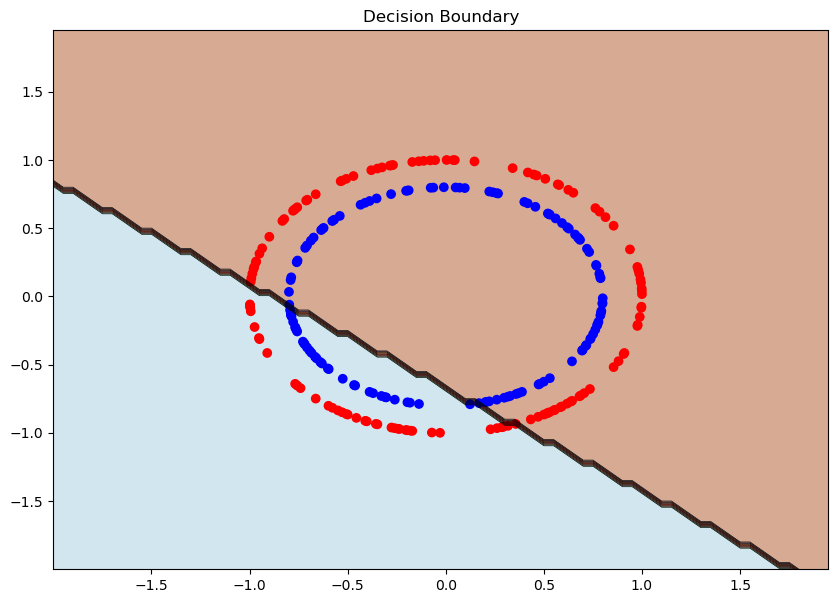
\includegraphics[width=\textwidth]{images/circles-linear-lr.png}
            \caption{ Linear Regression decision boundary on test set}
        \end{figure}
        {\fontsize{10pt}{12pt}\selectfont Linear SVM:} 
        \\ Test accuracy = 47.599999999999994 \%
        \\ Decision Boundary:
        \begin{figure}[H]
            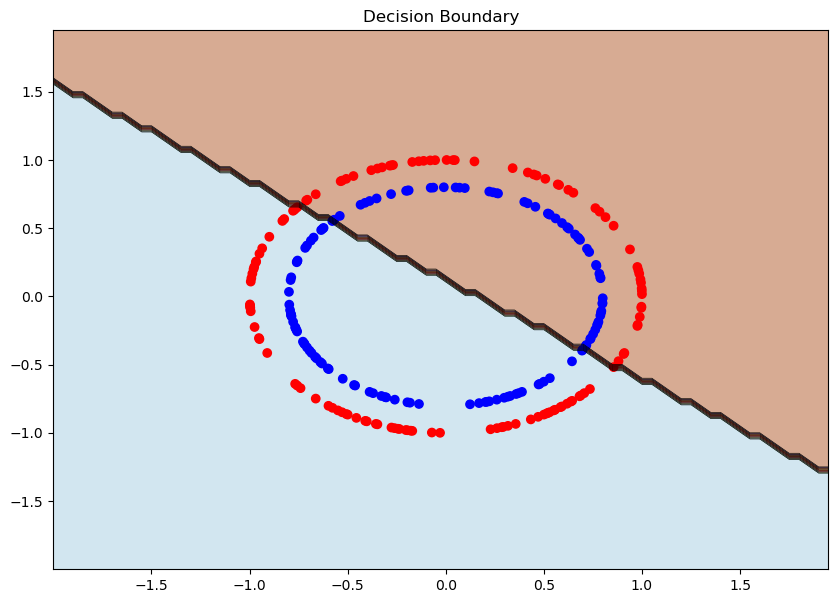
\includegraphics[width=\textwidth]{images/circles-linear-svm.png}
            \caption{ Linear Regression decision boundary on test set}
        \end{figure}
    \end{soln}
\item ( 5 pts) Show decision boundaries for Kernel SVM and Kernel Logistic Regression ( use rbf, polynomial
kernels). Try different values of hyperparameters, and report results with whichever works best.
\begin{soln}
    \\ After tring out different hyper parameters I chose the following.
    \\ {\fontsize{10pt}{12pt}\selectfont Linear Logistic Regression:} 
    \\ Test accuracy = 98.8\%
    \\
    {\fontsize{10pt}{12pt}\selectfont Linear SVM:} 
    \\ Test accuracy = 98.8\%
    \\
    \\ {\fontsize{10pt}{12pt}\selectfont Rbf Kernel Logistic Regression:}
    \\ I chose 50 samples to compute the kernel function with, I chose the $\gamma = 0.01$ and a step size = 0.05
    \\ Test accuracy = 100.0 \%
    \\ Decision Boundary:
    \begin{figure}[H]
        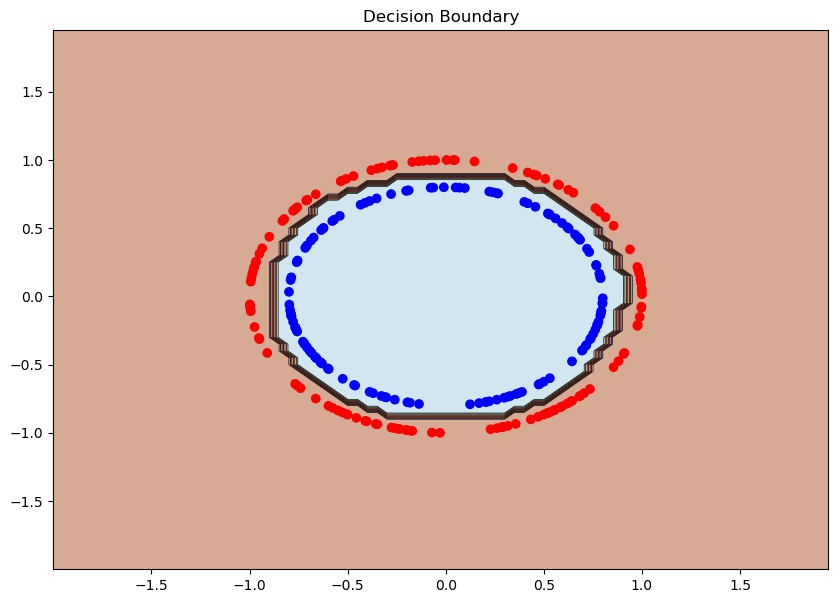
\includegraphics[width=\textwidth]{images/circles-rbf-lr.png}
        \caption{ Rbf Kernel Logistic Regression decision boundary on test set}
    \end{figure}
    {\fontsize{10pt}{12pt}\selectfont Polynomial Kernel Logistic Regression:} 
    \\ I chose 50 samples to compute the kernel function with, I chose the degree of the polynomial $d = 2$, polynomial constant $c = 1$ and a step size of 0.05
    \\ Test accuracy = 100.0 \%
    \\ Decision Boundary:
    \begin{figure}[H]
        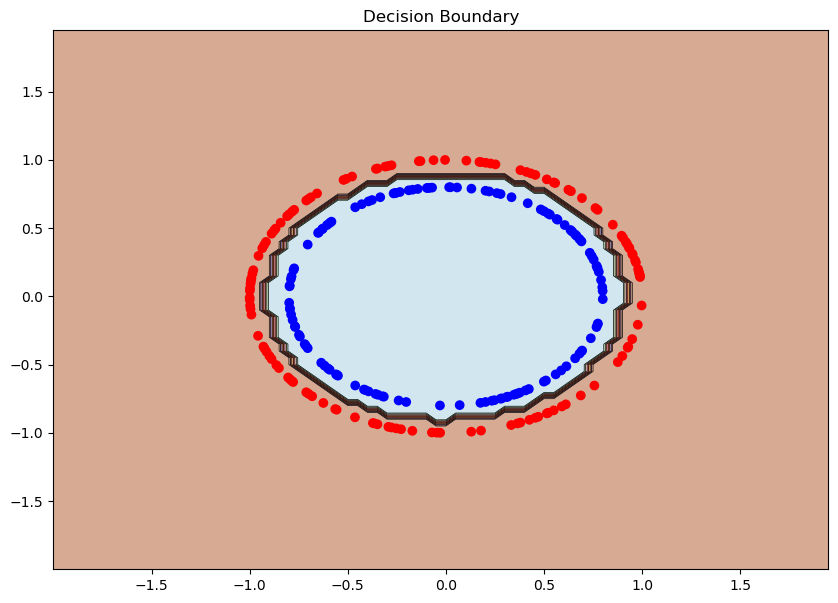
\includegraphics[width=\textwidth]{images/circles-poly-lr.png}
        \caption{ Polynomial Kernel Logistic Regression decision boundary on test set}
    \end{figure}
    {\fontsize{10pt}{12pt}\selectfont Rbf Kernel SVM:} 
    \\ I chose 50 samples to compute the kernel function with, I chose the $\gamma = \cfrac{1}{110}$, I chose the regularization parameter $C = 2.50$ and a step size of 0.05
    \\ Test accuracy = 100.0 \%
    \\ Decision Boundary:
    \begin{figure}[H]
        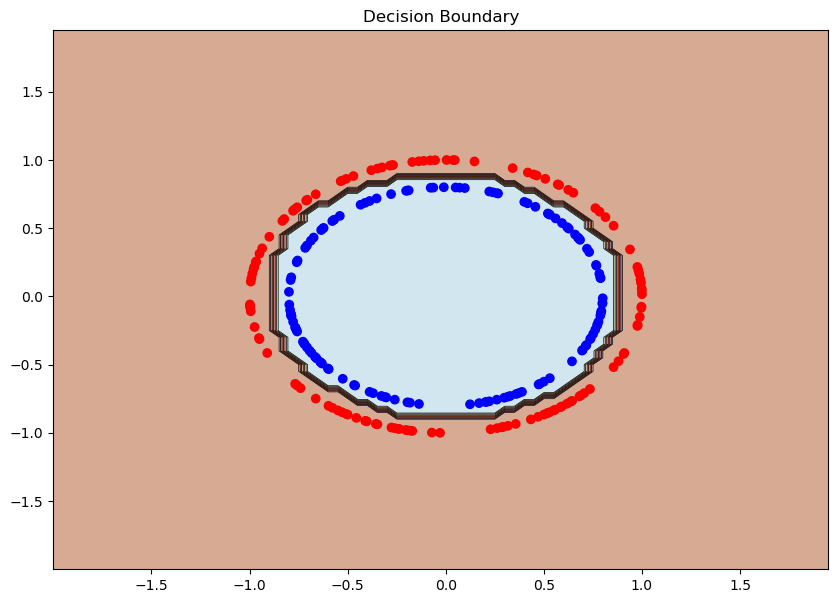
\includegraphics[width=\textwidth]{images/circles-rbf-svm.png}
        \caption{ Rbf Kernel SVM decision boundary on test set}
    \end{figure}
    {\fontsize{10pt}{12pt}\selectfont Polynomial Kernel SVM:}
    \\ I chose 50 samples to compute the kernel function with, I chose the degree of the polynomial $d = 2$, polynomial constant $c = 1$, I chose the regularization parameter $C = 1.50$ and a step size of 0.05
    \\ Test accuracy = 100.0 \%
    \\ Decision Boundary:
    \begin{figure}[H]
        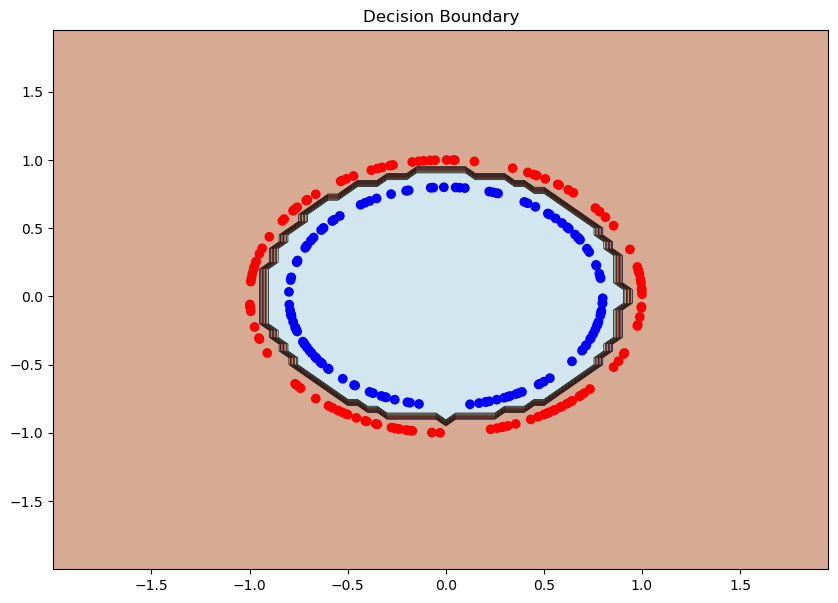
\includegraphics[width=\textwidth]{images/circles-poly-svm.png}
        \caption{ Polynomial Kernel SVM decision boundary on test set}
    \end{figure}
\end{soln}
\item ( 5 pts ) Train Neural Network from HW4, and $k$-NN classifiers on this dataset and show decision boundaries. ( You can use library implementation for these classifiers).
\begin{soln}
    {\fontsize{10pt}{12pt}\selectfont HW4 Neural Networl:} 
    \\ I chose step size of 0.05
    \\ Test accuracy = 51.6 \%
    \\ Decision Boundary:
    \begin{figure}[H]
        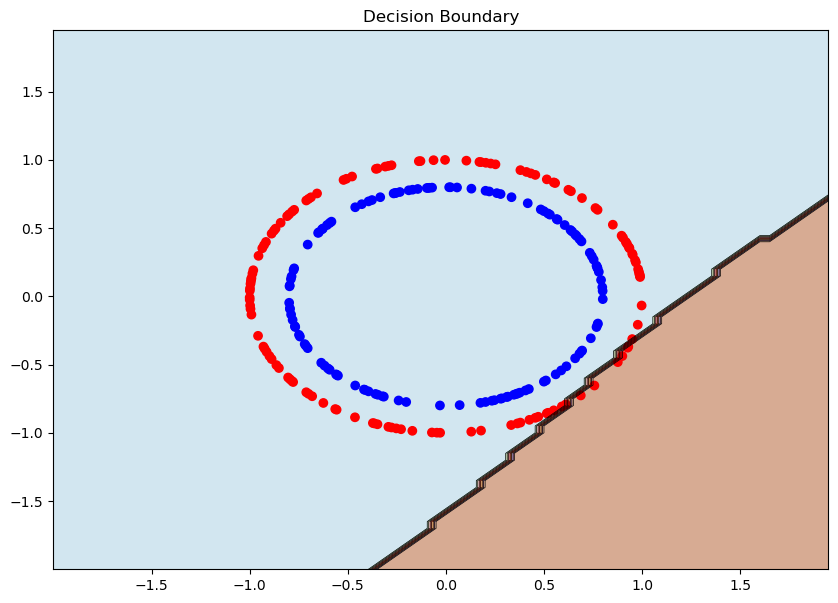
\includegraphics[width=\textwidth]{images/circles-hw4NN.png}
        \caption{ HW4 Neural Network boundary on test set}
    \end{figure}
    {\fontsize{10pt}{12pt}\selectfont $k$-NN on Circles dataset:}
    \\ I k=3 for this dataset as well since it gave me a good tradeoff between computation runtime and accuracy
    \\ Test accuracy = 100.0 \%
    \\ Decision Boundary:
    \begin{figure}[H]
        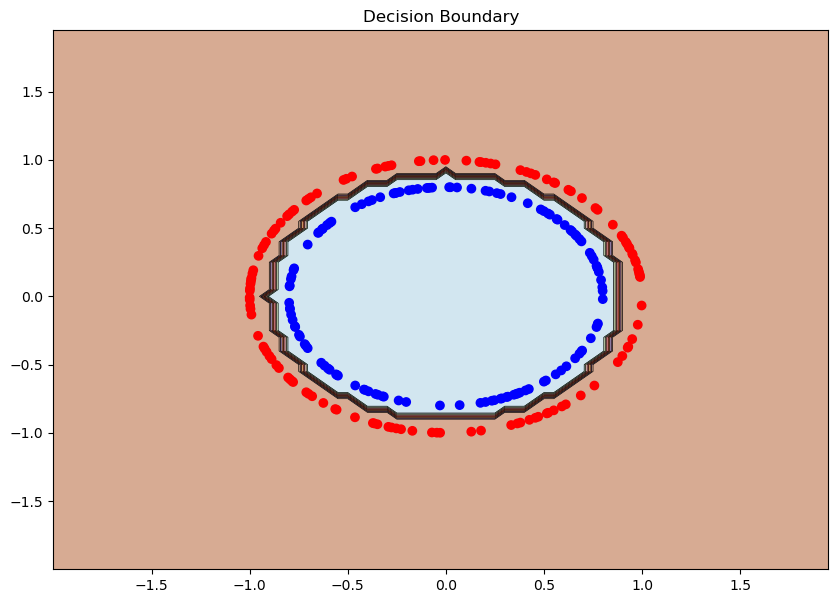
\includegraphics[width=\textwidth]{images/circles-kNN.png}
        \caption{ Polynomial Kernel SVM decision boundary on test set}
    \end{figure}
\end{soln}
\item ( 5 pts ) What are your conclusions from this exercise?
\end{enumerate}
\subsection{Evaluation on Real Dataset (20 pts)}
Let's put all this to some real use. For this problem, use the Wisconsin Breast Cancer dataset. You can download it from the sklearn library:
\begin{verbatim}
   sklearn.datasets.load_breast_cancer
\end{verbatim}
\begin{enumerate}
    \item  (10 pts) Do all the points of Section 3.3 in this dataset. Since these are high-dimensional data, you do not have to show the decision boundaries. Report test accuracies for these classifiers and discuss your findings.
    \begin{soln}
        \\ After tring out different hyper parameters I chose the following.\\
        \\ {\fontsize{10pt}{12pt}\selectfont Linear Logistic Regression:} 
        \\ Test accuracy = 96.842\%
        \\
        \\ {\fontsize{10pt}{12pt}\selectfont Linear SVM:} 
        \\ Test accuracy = 97.895\%
        \\
        \\ {\fontsize{10pt}{12pt}\selectfont Rbf Kernel Logistic Regression:}
        \\ I chose 50 samples to compute the kernel function with, I chose the $\gamma = \cfrac{10}{14}$ and a step size = 0.05
        \\ Test accuracy = 61.0526 \%
        \\
        \\ {\fontsize{10pt}{12pt}\selectfont Polynomial Kernel Logistic Regression:} 
        \\ I chose 50 samples to compute the kernel function with, I chose the degree of the polynomial $d = 1$, polynomial constant $c = 3$ and a step size of 0.05
        \\ Test accuracy = 61.0526 \%
        \\
        \\ {\fontsize{10pt}{12pt}\selectfont Rbf Kernel SVM:} 
        \\ I chose 50 samples to compute the kernel function with, I chose the $\gamma = \cfrac{1}{110}$, I chose the regularization parameter $C = 1.50$ and a step size of 0.05
        \\ Test accuracy = 100.0 \%
        \\
        {\fontsize{10pt}{12pt}\selectfont Polynomial Kernel SVM:}
        \\ I chose 50 samples to compute the kernel function with, I chose the degree of the polynomial $d = 6$, polynomial constant $c = 3$, I chose the regularization parameter $C = 1.50$ and a step size of 0.05
        \\ Test accuracy = 95.7895 \%
        \\
        \\ {\fontsize{10pt}{12pt}\selectfont HW4 Neural Networl:} 
        \\ I chose step size of 0.05
        \\ Test accuracy = 61.053 \%
        \\
        \\ {\fontsize{10pt}{12pt}\selectfont $k$-NN on Circles dataset:}
        \\ I k=5 for this dataset as well since it gave me a good tradeoff between computation runtime and accuracy. Increasing k further didn't significantly improve performance.
        \\ Test accuracy = 94.7368 \%
        \\
    \end{soln}
\item (10 pts) In addition, you also want to figure out the important features which determine the class. Which regularization will you use for this? Upgrade your SVM, Kernel SVM implementation to include this
regularization. Discuss the important features that you obtain by running your regularized SVM on this dataset. (You might need to normalize this dataset before training any classifier.)
\end{enumerate}
\end{document}
